%
%  Peter Vermeer
%
\documentclass[12pt,fullpage]{article}
\usepackage{fullpage}
\usepackage{psfrag}                                          % LaTeX graphics tool
\usepackage{pslatex}                                         % avoids the default cmr font
\usepackage{graphicx}                                        % graphics package 
\usepackage{epsfig}                                          % figures
\usepackage{hyperref}
\usepackage{color}

\begin{document}

\noindent
{\bf Benford distribution} (from \color{blue}\url{http://www.math.wm.edu/~leemis/chart/UDR/UDR.html}\color{black})

\noindent
The shorthand $X \sim {\rm Benford}$ is used to indicate that the
random variable $X$ has the Benford distribution.
A Benford random variable $X$ has probability mass function 
$$
f(x) = \log_{10}\left(1 + \frac{1} {x}\right) \qquad \qquad x = 1,2,\ldots,9.
$$
The probability mass function is illustrated below.

\begin{figure}[h!]
\begin{center}
\psfrag{labx}{$x$}
\psfrag{labf}{$f(x)$}
\includegraphics[width=3.6in]{BenfordPlot.ps}
\end{center}
\end{figure}

\noindent The cumulative distribution function on the support of $X$ is
$$
F(x) = P(X \le x) = \log_{10} (1+x) \qquad \qquad x = 1,2,\ldots,9.
$$
The survivor function on the support of $X$ is
$$
S(x) = P(X \ge x) = 1- \log_{10} x \qquad \qquad x = 1,2,\ldots,9.
$$
The hazard function on the support of $X$ is
$$
h(x) = \frac{f(x)}{S(x)} = \frac{\log_{10}\left(1+\frac{1}{x}\right)}{1- \log_{10}x}  \qquad \qquad x = 1,2,\ldots,9.
$$
The cumulative hazard function on the support of $X$ is
$$
H(x) = - \ln S(x) = -\ln (1- \log_{10}x)  \qquad \qquad x = 1,2,\ldots,9.
$$
The inverse distribution function is
$$
F ^ {-1}(u) = \lfloor 10^{u} \rfloor \qquad \qquad 0<u<1.
$$
%The moment generating function of $X$ is
%$$
%{\frac {{e^{t}} \left( \ln  \left( 2 \right) +{e^{t}}\ln  \left( 3 \right) -\ln  \left( 2 \right) {e^{
%t}}+2\,{e^{2\,t}}\ln  \left( 2 \right) -{e^{2\,t}}\ln  \left( 3 \right) +{e^{3\,t}}\ln  \left( 5
% \right) -2\,{e^{3\,t}}\ln  \left( 2 \right) +{e^{4\,t}}\ln  \left( 2 \right) +{e^{4\,t}}\ln  \left( 3
% \right) -{e^{4\,t}}\ln  \left( 5 \right) +{e^{5\,t}}\ln  \left( 7 \right) -{e^{5\,t}}\ln  \left( 2
% \right) -{e^{5\,t}}\ln  \left( 3 \right) +3\,{e^{6\,t}}\ln  \left( 2 \right) -{e^{6\,t}}\ln  \left( 7
% \right) +2\,{e^{7\,t}}\ln  \left( 3 \right) -3\,{e^{7\,t}}\ln  \left( 2 \right) +{e^{8\,t}}\ln 
% \left( 2 \right) +{e^{8\,t}}\ln  \left( 5 \right) -2\,{e^{8\,t}}\ln  \left( 3 \right)  \right) }{\ln 
% \left( 2 \right) +\ln  \left( 5 \right) }}
%$$

%\begin{eqnarray*}
%M(t) = -{\frac{1} {\ln \left( 2 \right) + \ln  \left( 5 \right) }} \kern 0.08 em 
%{{\rm e} ^ {t}} \left[ -\ln  \left( 2 \right) - {{\rm e} ^ {t}}
%\ln  \left( 3 \right) + \ln  \left( 2 \right) {{\rm e} ^ {t}} - 2 \, {{\rm e}
% ^ {2 \, t}} \ln \left(2 \right) + {{\rm e} ^ {2 \, t}} \ln \left(3 \right) -
%{{\rm e} ^ {3 \, t}} \ln \left(5 \right) & + &\\
%2 \, {{\rm e} ^ {3 \, t}} \ln \left(2 \right) - {{\rm e} ^ {4 \, t}} \ln \left(2 \right) - {{\rm e} ^ {4 \, t}} \ln \left(3 \right) + {{\rm e} ^{ 4 \, t}} \ln  \left(5 \right) - {{\rm e} ^ {5 \, t}} \ln  \left(7 \right) + {{\rm e} ^ {5 \, t}} \ln \left(2 \right) + {
%{\rm e} ^ {5 \, t}} \ln  \left(3 \right) - 3 \, {{\rm e} ^ {6 \, t}} \ln \left(2 \right) &+&\\ 
%{{\rm e} ^ {6 \, t}} \ln \left(7 \right) - 2 \, {{\rm e} ^ {7 \, t}} \ln \left(3 \right) + 3 \, {{\rm e} ^ {7 \, t}} \ln \left(2 \right) - {{\rm e} ^ {8 \, t}} \ln \left(2 \right) - {{\rm e} ^ {8 \, t}} \ln \left(5 \right) + 2 \, {{\rm e} ^ {8 \, t}} \ln \left(3 \right) \right]  \qquad \qquad -\infty < t < &\infty.&
%\end{eqnarray*}

\noindent The population mean, variance, skewness, and kurtosis  of $X$ is approximated with results from APPL
$$
E[X] = \frac{2\ln(2)-4\ln(3)+8\ln(5)-\ln(7)}{\ln(2)+\ln(5)}\cong 3.4402
$$
$$
V[X] \cong 6.0565 \qquad \qquad 
E\left[ \left( \frac{X - \mu}{\sigma} \right) ^ 3 \right] \cong 0.7956 \qquad \qquad 
E\left[ \left( \frac{X - \mu}{\sigma} \right) ^ 4 \right] \cong 2.4518.
$$

\vspace{0.1in}

%   X := [[log[10](1 + 1 / x)], [1 .. 9],["Discrete", "PDF"]];
\noindent
{\bf APPL verification:}
The APPL statements
\begin{verbatim}
X := BenfordRV();
Mean(X);
Variance(X);
Skewness(X);
Kurtosis(X);
MGF(X);
\end{verbatim}
verify the population mean, variance, skewness, kurtosis and moment generating function.
\end{document}
